% Valentino Vranic
% Metody inzinierskej prace 2012/13

\documentclass{beamer}

%\usetheme{Warsaw}
\usetheme{Frankfurt}
%\usetheme{JuanLesPins}
%\usetheme{Goettingen}

%\usecolortheme{seahorse}
%\usecolortheme{dolphin}
%\usecolortheme{rose}
% https://deic.uab.cat/~iblanes/beamer_gallery/
\usecolortheme{seagull}

%\useoutertheme[]{sidebar}

\setbeamercovered{transparent}

\usepackage[slovak]{babel}
\usepackage[T1]{fontenc}
\usepackage[utf8]{inputenc}
\usepackage{url}

\usepackage{listings}


\lstset{language=C++,basicstyle=\fontsize{8}{9.6}\selectfont,showstringspaces=false,columns=fullflexible,identifierstyle=\ttfamily,keywordstyle=\bfseries,showstringspaces=false,columns=fullflexible}
%\lstset{language=C,basicstyle=\fontsize{10.5}{12.6}\selectfont,identifierstyle=\ttfamily,keywordstyle=\bfseries,showstringspaces=false,columns=fixed}

\def\BibTeX{\textsc{Bib}\kern-.08em\TeX} 

\newcommand{\footcite}[1]{\footnote{\tiny #1}}
\newcommand{\umlet}{.5}
\newcommand{\emp}[1]{\textit{\alert{#1}}}
\newcommand{\kw}[1]{\mbox{\textbf{#1}}}
\newcommand{\id}[1]{\texttt{#1}}
\newcommand{\stl}{\guillemotleft}
\newcommand{\str}{\guillemotright}

\newcommand{\lsti}{\lstinline[basicstyle=\fontsize{10.5}{12.1}\selectfont]}

\newcommand{\ssection}[1]{
	\section{#1}
	\begin{frame}[fragile=singleslide]\frametitle{}
	\Huge #1
	\end{frame}
}

\newcommand{\ssectionn}[1]{
	\section*{#1}
	\begin{frame}[fragile=singleslide]\frametitle{}
	\Huge #1
	\end{frame}
}

\newenvironment{program}{\begin{beamercolorbox}[rounded=true,shadow=true]{block body}\vspace{-4mm}}{\vspace{-2mm}\end{beamercolorbox}}

\setbeamercolor{fvystup}{fg=white,bg=black}
\newenvironment{vystup}{\begin{beamercolorbox}[rounded=true,shadow=true]{fvystup}}{\end{beamercolorbox}}

\newenvironment{poznamka}{\begin{beamercolorbox}[rounded=true,shadow=false]{block body}}{\end{beamercolorbox}}

\setbeamertemplate{footline}[page number]
{
%\insertpagenumber
%\begin{beamercolorbox}{section in head/foot}
%\vskip2pt\insertnavigation{\paperwidth}\vskip2pt
%\end{beamercolorbox}%
}



\author{Timon Lumír Fillo}
%\url{www.fiit.stuba.sk/~vranic}, \url{vranic@fiit.stuba.sk}}
%{\tiny \url{www.fiit.stuba.sk/~vranic}, \url{vranic@fiit.stuba.sk}}
\institute{
	Ústav informatiky, informačných systémov a softvérového inžinierstva\\
	Fakulta informatiky a informačných technológií\\
	Slovenská technická univerzita v Bratislave}

\subtitle{\vspace{3mm} Metódy inžinierskej práce 2024/2025}

\title{Spotify recommendation system and its flwas
}

\date{\footnotesize 22. Október 2024}




\begin{document}

\begin{frame}[fragile=singleslide]
\titlepage
\end{frame}


\begin{frame}[fragile=singleslide]\frametitle{Prehľad}
\tableofcontents
\end{frame}

\section{Úvod}
\begin{frame}[fragile=singleslide]\frametitle{Digitalizácia hudby}
\begin{itemize}
	\item Prístup k hudbe sa vďaka internetu rozšíril na celý svet
	\item Umožnili tomu hlavne streamovacie platformy ako napríklad Spotify, Youtube Music a Apple Music
	\item Umelci teraz môžu osloviť publikum na celom svete, čím sa otvárajú nové príležitosti na trhu hudby
\end{itemize}
\end{frame}

\section{Globalizácia hudby}
\begin{frame}[fragile=singleslide]\frametitle{Dosah hudby a jej vplyv}
\begin{itemize}
	\item Umelci svoju hudbu môžu zdieľať s kýmkoľvek pripojeným na internet
	\item Objavili sa nové trhy s hudbou, vďaka ktorým sa menším umelcom ľahšie darí.
	\item Táto zmena urobila z hudby skutočne globálny priemysel
\end{itemize}
\end{frame}

\begin{frame}[fragile=singleslide]
\begin{figure}
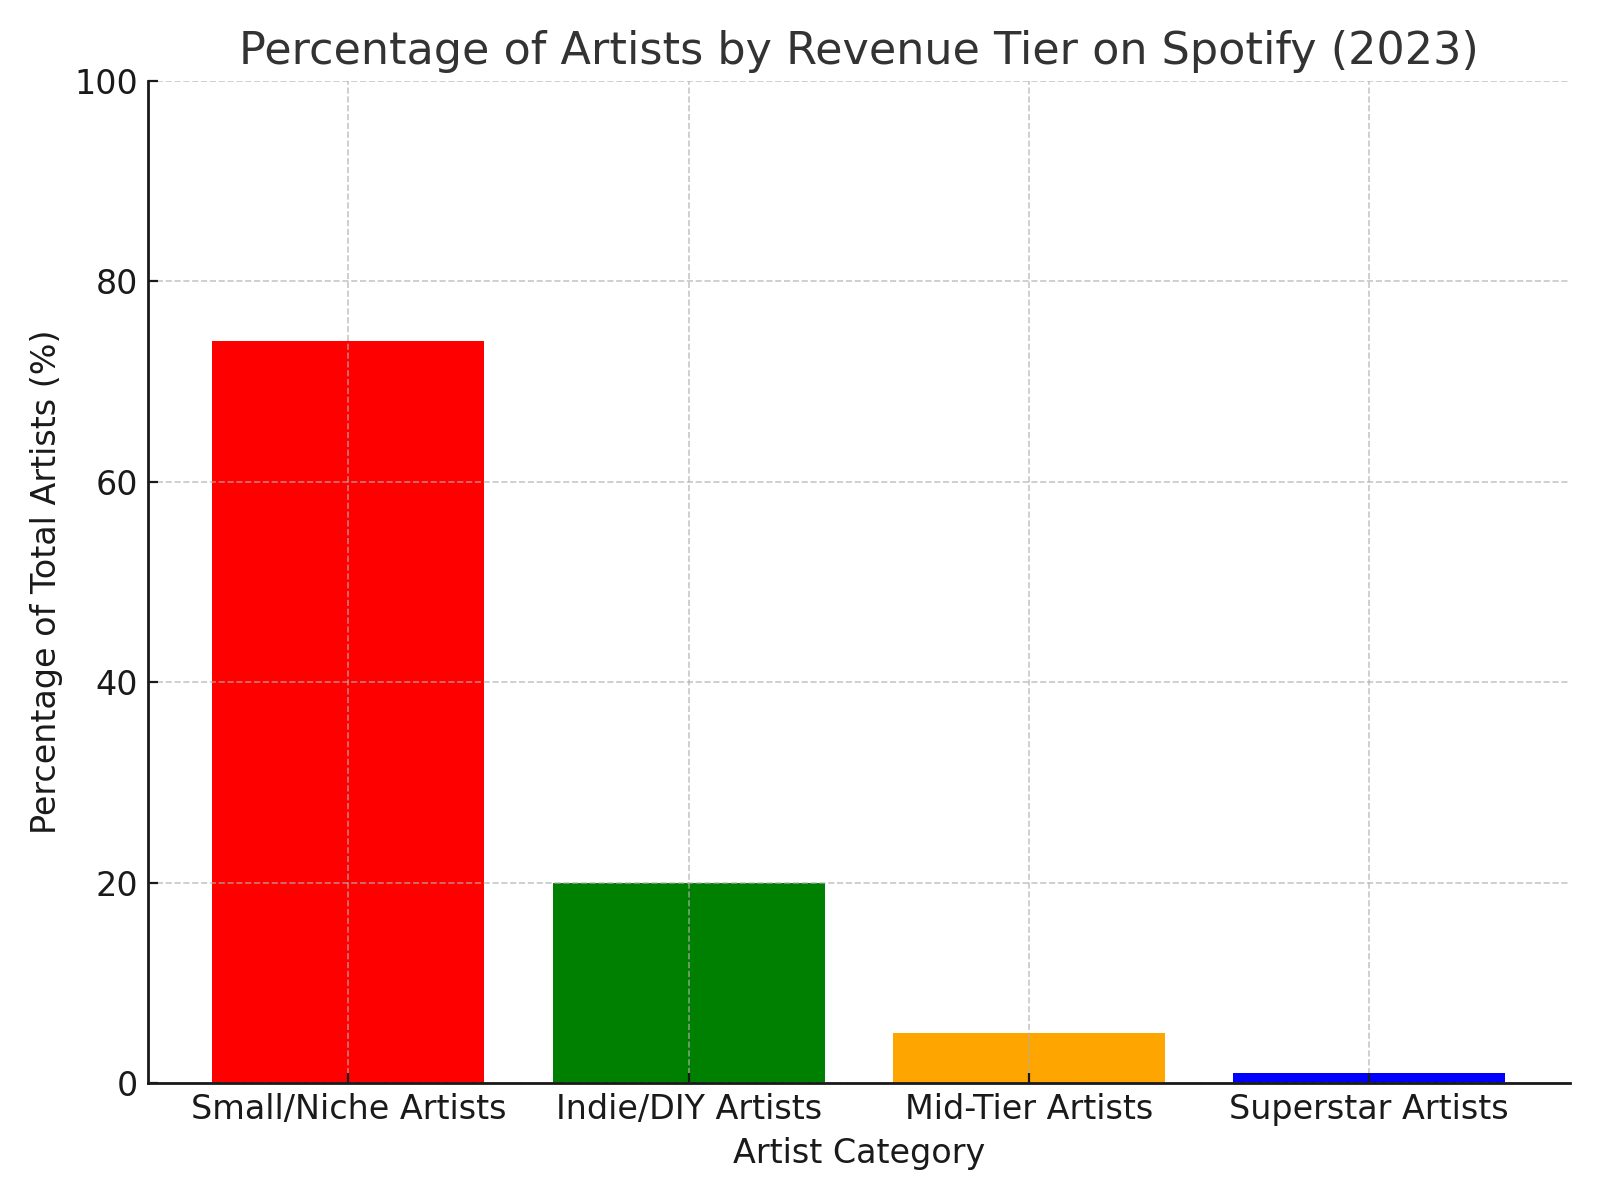
\includegraphics[width=0.7\linewidth]{graphics/spotify_revenue_graph.png}

\begin{table}[htb]
\centering
\resizebox{0.8\linewidth}{!}{

\begin{tabular}{|l|c|c|c|}
\hline
\textbf{Artist Category} & \textbf{Monthly Listeners} & \textbf{Estimated Yearly Earnings} & \textbf{\% of Total Artists} \\ \hline
Superstar Artists    & 5M+             & \$1M+              & <1\% \\\hline
Mid-Tier Artists     & 500K-5M         & \$100K - \$1M      & 5\% \\\hline
Indie/DIY Artists    & 100K-500K       & \$10K - \$100K     & 20\% \\\hline
Small/Niche Artists  & <100K           & <\$10K              & 74\% \\\hline
\end{tabular}
}

\end{table}
\caption{Úrovne výnosov zo streamovania interpretov na Spotify !CITETHIS!}
\end{figure}
\end{frame}


\end{document}

% príkaz \ssection by vytvoril zvláštný slajd s názvom časti - v krátkych prezentáciách to prekáža, lebo oberá o čas
\section{Odrazky}
\begin{frame}[fragile=singleslide]\frametitle{Nejaký slajd}
\begin{itemize}
\item Odrážky na prvej úrovni
\item Môže ich byť viac
	\begin{itemize}
	\item Toto je už druhá úroveň
	\item Ďalšia odrážka
	\end{itemize}
\item Pokračuje prvá úroveň
\end{itemize}
\end{frame}

\section{Obrazok}
\begin{frame}[fragile=singleslide]\frametitle{Logo fiit}